\chapter{Réalisations}
\label{AnalyseConception}

\section{Environnement de travail}
Environnement de travail =
Windows 8.1 Profesionnal (machine hôte)
Machine virtuelle de développement via VirtualBox (Windows Server 2012 R2 Standard)

Outils/Projets =
DataWizard (python) = génération de réseau de transports multi-modaux
OneBusAway (java) = traitement de données de transport (standard GTFS)

Gestion de projets =
Redmine (gestion des tickets = bugtracker)
eGroupware (intranet)
SVN (gestion des codes sources)

IDE =
    Liclipse (python)
    Eclipse Mars (java)

SGBD = 
Postgresql/Postgis

\section{Les Projets}

\subsection{MobiSaaS}

\paragraph{Présentation}

Le projet MobiSaaS s'inscrit dans la démarche d'entreprise de proposer des solutions en mode \textbf{SAAS}. Le projet consiste d'une manière générale à exposer les fonctionnalité de la solution desktop du produit "MobiAnalyst"(cf. Figure ~\ref{fig:Offre du produit MobiAnalyst}).
\begin{figure}[!h]\label{fig:Offre du produit MobiAnalyst}
\centering
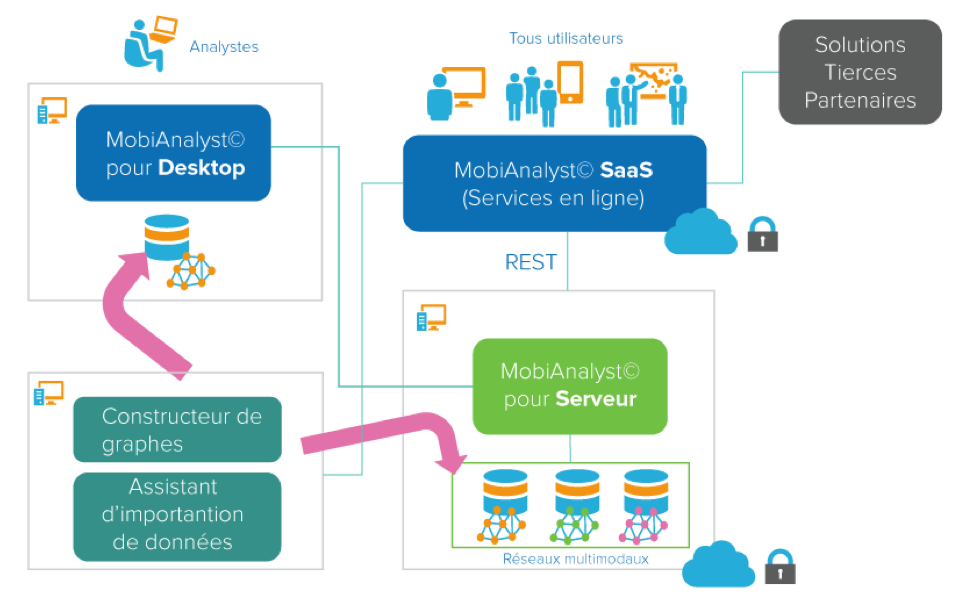
\includegraphics[width=12cm]{images/offre_MobiAnalyst.png}
\caption{Offre du produit MobiAnalyst}
\end{figure} 

\paragraph{Technologies}

\paragraph{Réalisations}

\paragraph{Perspectives}

\subsection{DataWizard}

\paragraph{Présentation}

\paragraph{Technologies}

\paragraph{Réalisations}
Parmi les missions effectuées au cours du stage, il y en a eu une directement liée à ce contexte de développement d’applications. Il s’agissait de tests effectués sur le module Datawizard (Python / SQL), qui permet la création de réseaux MobiAnalyst.\\

\paragraph{Perspectives}
